\documentclass[xpsejal00-gcc-plugin.tex]{subfiles}
\begin{document}

\chapter{State of the Art}
\label{chap:sota}

This chapter provides a detailed account of the existing Code Listener infrastructure in the Predator repository~\cite{PredatorSuite2016,PredatorHP2020} and as described in the original publication~\cite{CodeListener2012}. Understanding the design decisions and limitations of the current implementation is necessary background for the design choices made in this thesis.

\section{Overview}

The Code Listener infrastructure was originally developed at the Faculty of Information Technology, Brno University of Technology, as a support library for the Predator and Forester research prototype analyzers~\cite{CodeListener2012}. Its central goal is to \emph{decouple} the static analysis logic from the internals of particular compilers. Compilers such as GCC expose rich intermediate representations (IRs), but their internal APIs are large, poorly documented in places, and subject to change across versions. Code Listener provides a concise, well-documented C++ API that absorbs this complexity and exposes a stable interface to analyzer authors.

From the perspective of an analyzer, Code Listener behaves like a black box: the analyzer registers itself, a \emph{GCC plug-in} is loaded, and when GCC finishes compiling a translation unit, the analyzer finds a fully populated \emph{code storage} object ready to inspect. The analyzer never needs to call a GCC API directly.

\section{GCC and the Plug-in Interface}
\label{sec:gcc-plugin}

GCC is a collection of compilers for C, C++, Fortran, Ada, Go, and other languages, organized around a three-phase design. A~\emph{front end} that parses source code and produces an abstract syntax tree (AST), a \emph{middle end} that performs language-independent optimizations on several IR levels, and a \emph{back end} that generates machine code~\cite{GCCInternals}. The plug-in interface~\cite{GCCPluginAPI} allows client code to register callbacks at well-defined points in the compilation pipeline, such as after parsing, after each optimization pass, after each function is compiled, and so on.

Code Listener registers a callback that fires once per function. This occurs after the front end produces the function's GIMPLE IR, but before the optimizer runs significant transformations. At this stage, the IR is in \emph{low-level GIMPLE} form. This form uses a three-address representation, where expressions become sequences of simple assignments, unary and binary operations, calls, and control-flow instructions.

\subsection{GIMPLE Intermediate Representation}
\label{sec:gimple}

GIMPLE is the principal IR used by GCC's middle end~\cite{GCCInternals}. In GIMPLE, each function is represented as a \emph{control flow graph} (CFG) whose nodes are \emph{basic blocks}, sequences of instructions that execute without intervening branches. Edges represent possible transitions between blocks. Instructions in low-level GIMPLE are restricted to a three-address form. Each instruction reads at most two operands and writes at most one result. Compound expressions are split into sequences by introducing temporary variables so as not to break the three-address form.

GIMPLE recognizes, and Code Listener exposes the following instruction kinds:

\begin{description}
  \item[\texttt{UNOP}] A~unary operation of the form $\mathit{dst} := \circ\, \mathit{src}$, where $\circ$ is the identity (assignment), logical not, bitwise not, or unary minus.
  \item[\texttt{BINOP}] A~binary operation $\mathit{dst} := \mathit{src}_1 \circ \mathit{src}_2$ supporting comparison, arithmetic (including pointer arithmetic), logical, and bitwise operators.
  \item[\texttt{CALL}] A~function call $\mathit{dst} := f(\mathit{arg}_1, \ldots, \mathit{arg}_n)$, where $f$ may be a statically known function, an external function, or a function pointer. A~\texttt{CALL} is treated as a \emph{non-terminal} instruction, which means that it may appear in the middle of a basic block.
  \item[\texttt{JMP}] An unconditional branch to a single target block, which is always terminal.
  \item[\texttt{COND}] A~conditional branch with a Boolean operand and two targets (\emph{then} and \emph{else}), also always terminal.
  \item[\texttt{SWITCH}] A~generalization of \texttt{COND} for integer or enumerated operands, specifying a list of value--target pairs and a default target; always terminal.
  \item[\texttt{RET}] A~function return carrying an optional return value, always terminal, marks an endpoint of the CFG.
  \item[\texttt{ABORT}] An unconditional program termination, inserted after calls to \texttt{noreturn} functions such as \texttt{abort()} from \texttt{<stdlib.h>}, which is also always terminal.
\end{description}

\subsection{Operands and Accessors}

The key structural element of both the GCC adapter API and the code storage API is the \emph{operand}, represented by the C structure \texttt{cl\_operand}. An operand is either void (no value), a constant (\texttt{cl\_cst}), or a variable (\texttt{cl\_var}). Constants cover numeric literals, string literals, and function addresses. Variables carry a scope tag (global, static, or local) and a unique integer identifier (\emph{uid}) that is globally unique within a translation unit when using the GCC front end.

Operands are augmented by a chain of \emph{accessors} (\texttt{cl\_accessor}) that modify the semantics of the base operand~\cite{CodeListener2012}:

\begin{itemize}
  \item \textbf{Reference} (\texttt{CL\_ACCESSOR\_REF}): take the address of the operand.
  \item \textbf{Dereference} (\texttt{CL\_ACCESSOR\_DEREF}): load the value at the pointer.
  \item \textbf{Array item} (\texttt{CL\_ACCESSOR\_DEREF\_ARRAY}): index into an array.
  \item \textbf{Struct item} (\texttt{CL\_ACCESSOR\_ITEM}): access a field of a composite type.
\end{itemize}

The accessor chain is subject to structural constraints: a dereference, if present, must appear at the beginning of the chain, and a reference, if present, must appear at the end. Chained dereferences are forbidden. If a C expression would require multiple pointer indirections in one operand, Code Listener splits it into a sequence of instructions, each with at most one dereference. This design keeps the instruction set small while covering all C language pointer and aggregate semantics.

\subsection{Type System}

Since C is statically typed, every operand and accessor carries a reference to a \texttt{cl\_type} structure that describes the compile-time type. A~\texttt{cl\_type} is characterized by its \emph{kind} (integer, floating-point, pointer, array, struct, union, function type, void, etc.) and, for non-atomic types, by an array of \texttt{cl\_type\_item} references that describe the constituent sub-types or fields. Struct and union items additionally carry a byte \emph{offset} from the start of the containing object. All types, variables, and functions are assigned globally unique long integer uids, which Code Listener exposes for use as dictionary keys or for identifying entities across compilation units.

\section{Architecture of the Original Code Listener}
\label{sec:cl-architecture}

\begin{figure}[h]
  \centering
  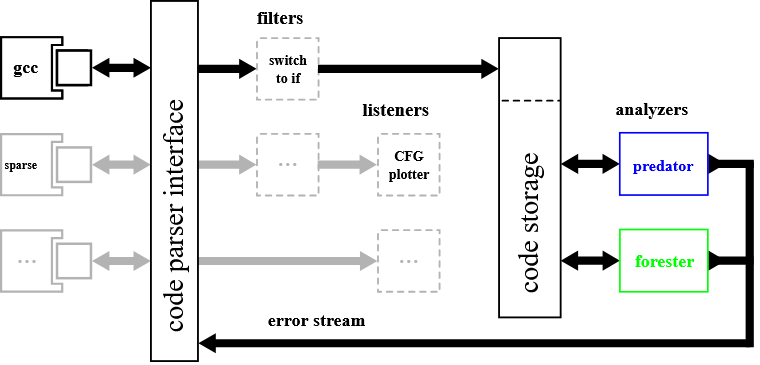
\includegraphics[width=0.85\textwidth]{obrazky-figures/old_architecture}
  \caption{Block diagram of the original Code Listener infrastructure (reproduced from~\cite{CodeListener2012}). Data flows left to right: adapters translate each compiler's internal IR into a stream of listener callbacks. Filters and listeners process that stream. Code storage accumulates the result into a persistent object model.}
  \label{fig:old-arch}

\end{figure}

Figure~\ref{fig:old-arch} shows the high-level structure of the original Code Listener. Three conceptual layers are present: the \emph{code parser interface}, the \emph{filter and listener pipelines}, and the \emph{code storage}.

\subsection{Code Parser Interface and Adapters}

The \emph{code parser interface} is specified entirely in plain C (the header \texttt{cl/code\_listener.h}) so that it can be consumed by code parsers written in C, for example, Sparse, the Linux kernel's semantic analysis tool, which uses certain C++ keywords as identifiers in its own headers~\cite{CodeListener2012}. The interface consists of a set of callback function pointers that the adapter calls in a prescribed order as it traverses the compiler's internal data structures.

An \emph{adapter} is a small component embedded inside each supported compiler. It is responsible for translating the compiler-specific IR into a sequence of calls to the Code Listener API. Two adapters were shipped with the original distribution: one for GCC (the primary adapter, supporting both C and C++~\cite{CppExtension2014}) and one for Sparse. A~third adapter for Clang/LLVM was contributed as a bachelor's thesis~\cite{LLVMAdapter2014}.

The adapter invokes the callbacks in a well-defined order corresponding to a depth-first traversal of the program. Specifically, it opens a namespace, a type, a function, a basic block, emits instructions one by one, closes the block, closes the function, closes the namespace, and so forth. The listener on the other side of the API can therefore reconstruct the complete program structure by maintaining a stack.

\subsection{Filters}

A~\emph{filter} is a component that sits between an adapter and a downstream listener. It implements the same callback interface on both its input and its output, intercepts the incoming stream of events, optionally transforms them, and re-emits them downstream. Filters can be chained. The original distribution ships one filter that is unconditionally active in all predefined configurations: the \emph{switch-to-if} filter, which translates every \texttt{SWITCH} instruction into an equivalent sequence of \texttt{COND} instructions. This means that the code storage and all analyzers built on it never observe \texttt{SWITCH} instructions, regardless of whether the original source code contained any.

\subsection{Listeners}

Beyond code storage, Code Listener also exposes the listener interface to diagnostic tools. A~\emph{listener} uses the same input-side callback API but does not re-emit the stream; instead, it processes it in place. The original distribution includes a CFG plotter (\texttt{cl\_dotgen}) that generates Graphviz visualizations of control flow graphs, and an intermediate code printer (\texttt{cl\_pp}) that produces a textual dump of the three-address IR.

\subsection{Code Storage}
\label{sec:code-storage}

The \emph{code storage} is a special listener that, rather than processing the stream on the fly, accumulates the incoming events into a persistent, navigable object model. Once the entire program has been pushed through the pipeline, an analyzer can query this model at will.

The top-level object is named \texttt{Storage}. It contains three lookup containers: \texttt{TypeDb} (all types encountered in the program), \texttt{VarDb} (all variables), and \texttt{FncDb} (all functions). Each function is represented by a \texttt{Fnc} value that provides the function's argument list, its local variable list, and its CFG. The CFG is a \texttt{ControlFlow} object that can be iterated as a collection of \texttt{Block} values, each of which holds an ordered sequence of \texttt{Insn} (instruction) values. Instructions store their operands and branch targets in \texttt{std::vector} containers. Every significant object, that being a type, variable, function, or instruction, carries a \texttt{cl\_loc} location structure that records the corresponding source file name, line number, and column, so that an analyzer can report errors in the standard GCC diagnostic format.

\section{Mandatory Pre-Analysis Steps}
\label{sec:mandatory-analyses}

Before handing control to the registered analyzer, the existing Code Listener infrastructure unconditionally executes four analysis passes that further transform or annotate the code storage:

\begin{enumerate}
  \item \textbf{Call graph construction.} A~call graph is built by scanning all \texttt{CALL} instructions in the code storage. The graph is then made available through the \texttt{Storage} object.
  \item \textbf{Loop-closing edge annotation.} The CFG of each function is examined to identify \emph{back edges}, meaning the edges that lead to a previously-visited basic block, and these are annotated to assist analyses that need to distinguish loop-entry points from other join points.
  \item \textbf{Points-to analysis.} A~flow-insensitive, context-insensitive points-to analysis is run over the code storage to compute approximate pointer target sets for each variable.
  \item \textbf{Liveness analysis.} A~standard backward liveness analysis is computed per function. Each instruction in the code storage is extended with a bit vector recording which variables can be killed at that point.
\end{enumerate}

All four passes are non-optional. They execute for every invocation of Code Listener, regardless of whether the registered analyzer actually uses their results. There is no mechanism for an analyzer to opt out of a pass or to request a different analysis in its place.

\section{Existing Adapters and Extensions}

Since its initial release, Code Listener has been extended by several student projects at FIT BUT:

\begin{itemize}
  \item \textbf{Sparse adapter} (master's thesis, Jan Pokorný, 2012)~\cite{SparseAdapter2012}: an adapter for the Sparse semantic checker used in Linux kernel development. Sparse is written in C and serves as a lightweight alternative front end.
  \item \textbf{LLVM/Clang adapter} (bachelor's thesis, Veronika Šoková, 2014)~\cite{LLVMAdapter2014}: an adapter that hooks into the Clang/LLVM compilation pipeline and feeds the LLVM IR into the Code Listener callback interface. This adapter was later integrated into the main Predator distribution as an official alternative front end.
  \item \textbf{C++ support for the GCC adapter} (bachelor's thesis, David Kašpar, 2014/2015)~\cite{CppExtension2014}: an extension of the GCC adapter that handles GCC's representation of C++ constructs, these being virtual methods, destructors, and name mangling, so that Predator and Forester can analyze C++ programs.
\end{itemize}

\section{Limitations of the Existing Architecture}
\label{sec:limitations}

The original Code Listener architecture was a significant practical achievement when it was designed. It successfully decoupled Predator and Forester from GCC, enabled the LLVM and Sparse adapters, and supported analysis of real industrial code. However, as the tool suite has grown, several structural limitations have become apparent:

\begin{description}
  \item[Mandatory, non-optional transformations.] The switch-to-if filter always executes. An analyzer that directly supports \texttt{SWITCH} instructions cannot accept the unmodified IR.
  \item[Mandatory, non-optional pre-analyses.] The four analyses described in Section~\ref{sec:mandatory-analyses} always run, consuming time and memory even when the registered analyzer does not need results. There is no partial evaluation or lazy initialization.
  \item[No standardized annotation mechanism.] Analyzers that wish to attach their own data to code model entities must maintain their own side tables with no infrastructure support.
  \item[No structured query API.] Iterating over the code model requires direct traversal through nested C++ containers. There is no abstraction for common access patterns.
  \item[No uniform export interface.] Producing output in structured formats (JSON, DOT) requires ad-hoc code in each analyzer.
  \item[GCC version coupling.] The adapter code uses several GCC-internal APIs that change across major GCC versions. Upgrading the GCC toolchain has historically required patching the adapter~\cite{PredatorHP2020}.
\end{description}

These limitations motivate the redesign described in the following chapter.

\end{document}
